\documentclass[]{final_report}
\usepackage{graphicx}
\usepackage{hyperref}


%%%%%%%%%%%%%%%%%%%%%%
%%% Input project details
\def\studentname{Luke Sell}
\def\reportyear{2019}
\def\projecttitle{Playing Games and Solving Puzzles Using AI}
\def\supervisorname{Iddo Tzameret}
\def\degree{BSc (Hons) in Computer Science}
\def\fullOrHalfUnit{Full Unit} % indicate if you are doing the project as a Full Unit or Half Unit
\def\finalOrInterim{Presentation} % indicate if this document is your Final Report or Interim Report

\begin{document}

\maketitle

{ \huge \bfseries {
		Introduction:
		
		The aim of this Project is to show how AI can be used to solve a puzzle, in this case Sudoku.
		
		Sudoku is a puzzle easily solvable by AI, there is only one solution and three rules.
		
		Therefore Sudoku can be modelled as a Constraint Satisfaction Problem, where one state can is not compatible with another.
		
		A simple algorithm would be able to search for this solution and backtracking if any of the states is not valid.
		
		Constraint propagation allows such algorithms to solve puzzles very quickly and efficiently.
		
		\newpage
		What I have achieved:
		\newline
		Programs:
		
		I have written my program in C++ and using the SDL framework to display the GUI, have created a Main menu and puzzle screen that allows the user to navigate and use my application to play and solve Sudoku.
		
		I started development of my AI solver by first solving the N Queens problem, this involved creating a backtracking algorithm that would find a state where the Queens could be placed on the chessboard without being able to attack each other.
		\newpage
		This algorithm would start by attempting to place a Queen on the chessboard and then check these constraints and if this was valid it would move on to the next square if not it would remove the queen and then try the next square, if the algorithm had backtracked to an already valid Queen it would then remove it, as this state would not allow for all the queens to be placed.
		
		For Sudoku, I started by displaying the grid on the screen, to do this I rendered each square in its respective position and then rendered any overlays afterwards. The user is then able to select squares on the grid and enter any number, so that they can attempt to solve the puzzle themselves.
		
		To solve Sudoku I used a similar algorithm to the N Queens problem, once again a solution can be found using a backtracking algorithm and checking the constraints are satisfied, every square must be filled in with a number between one and nine. This is done by trying the first possible number for a square then moving on to the next square in the grid, then backtracking if a number is not valid and trying the next number until all numbers have been tried or a solution has been found.
		
		This was then extended so that the constraints are modelled with the possible values of a square being used and then eliminating numbers from these possible values as numbers are filled in on the grid.
		
		\newpage
		Reports:
		
		I have found many Design Patterns that are useful for my program, such as Strategy to represent many different AI solver algorithms, Iterator to be used when moving to the next square, Visitor to implement what the solver should do with different squares and Memento to keep track of a squares previous values.
		
		Sudoku can be solved by backtracking, a variation of a depth first search, Sudoku has an initial and a goal test and actions must be performed by a solver to find the next state, so that the goal state may be found. A backtracking search on a Sudoku puzzle will search up to the depth of 81 if possible before trying other branches, however as the constraints of the puzzle can be checked during the search, not all states in a branch have to be checked. This results in an algorithm that is very efficient in both time and memory used, having at most 81 instances stored, and is complete, always finding a solution if there is one.
		
		A Constraint Satisfaction Problem is modelled as having variables, domains of each variable and constraints between variables, Sudoku can be represented as such with each square being a variable, the domain being the numbers one to nine and the constraints being that a number cannot be repeated in a row, column or box. A variable can be made node consistent by eliminated all values in its domain that do not satisfy the variables unary constraints. A variable is arc consistent if all the values in its domain satisfy the variables binary constraints. This would mean that between two variables and for all values in the first variables domain there is a value in the second variables domain that satisfies the binary constraint on the arc joining them. This represents how constraint propagation can be modelled to reduce the possible numbers for all squares on a Sudoku grid and make solving the puzzle significantly easier.
		
		A human solver uses techniques similar to that of constraint propagation, that being the process of working out which numbers are valid for a square and using this to work out valid numbers for other squares, while also trying possible numbers then backtracking if this does not work.
		
		The UI for the solver displays the grid with lines separating the squares, these are dotted if in a box, the initial filled in squares are locked, displaying a grey overlay, and a selected square is highlighted in green, squares with the filled in number zero are shown as empty.
		
		An n\textsuperscript{2} x n\textsuperscript{2} Sudoku is NP complete, as the problem is in NP, it can be represented as a decision problem, there either being a solution that can be verified in polynomial time or no solution and NP hard, as Sudoku can be represented as a graph colouring problem which is known to be NP hard as there is a polynomial time many-one reduction of this to Sudoku which implies it is NP hard.
		
		%\newpage
		What I intend to achieve:
		\newline
		Programs:
		
		I will improving my program by implementing more design patterns such as flyweight to reuse number objects and state to represents the different GUI screens behaviours.
		
		I will extend my program by allowing the user to generate new Sudoku puzzles by creating a filled in grid by randomly placing numbers that satisfy the constraints then removing as many numbers as possible while still only allowing one solution. I will also allow the user to save and load puzzles from files.
		
		I will also improve the AI solving algorithm to make it more efficient, using dynamic variable ordering, backjumping and other optimizations.
		
		I will also improve the GUI so that the user can make notes of possible numbers in squares, so that they can keep track of constraint propagation like the solver.
		
		I will also allow the user to modify the application settings to use different screen sizes, use a timer and set different grid sizes.
		
		%\newpage
		Reports:
		
		I will describe the software engineering principles I have used, such as documenting my code, using a repository and unit tests.
		
		I will also describe the usage of data structures and there performance impact on time and memory.
		
		I will also describe the CSP and optimizations for it.
		
		\newpage
}}

\newpage

\begin{figure}[h]
	\centering
	\fboxsep 2mm
	\framebox{
		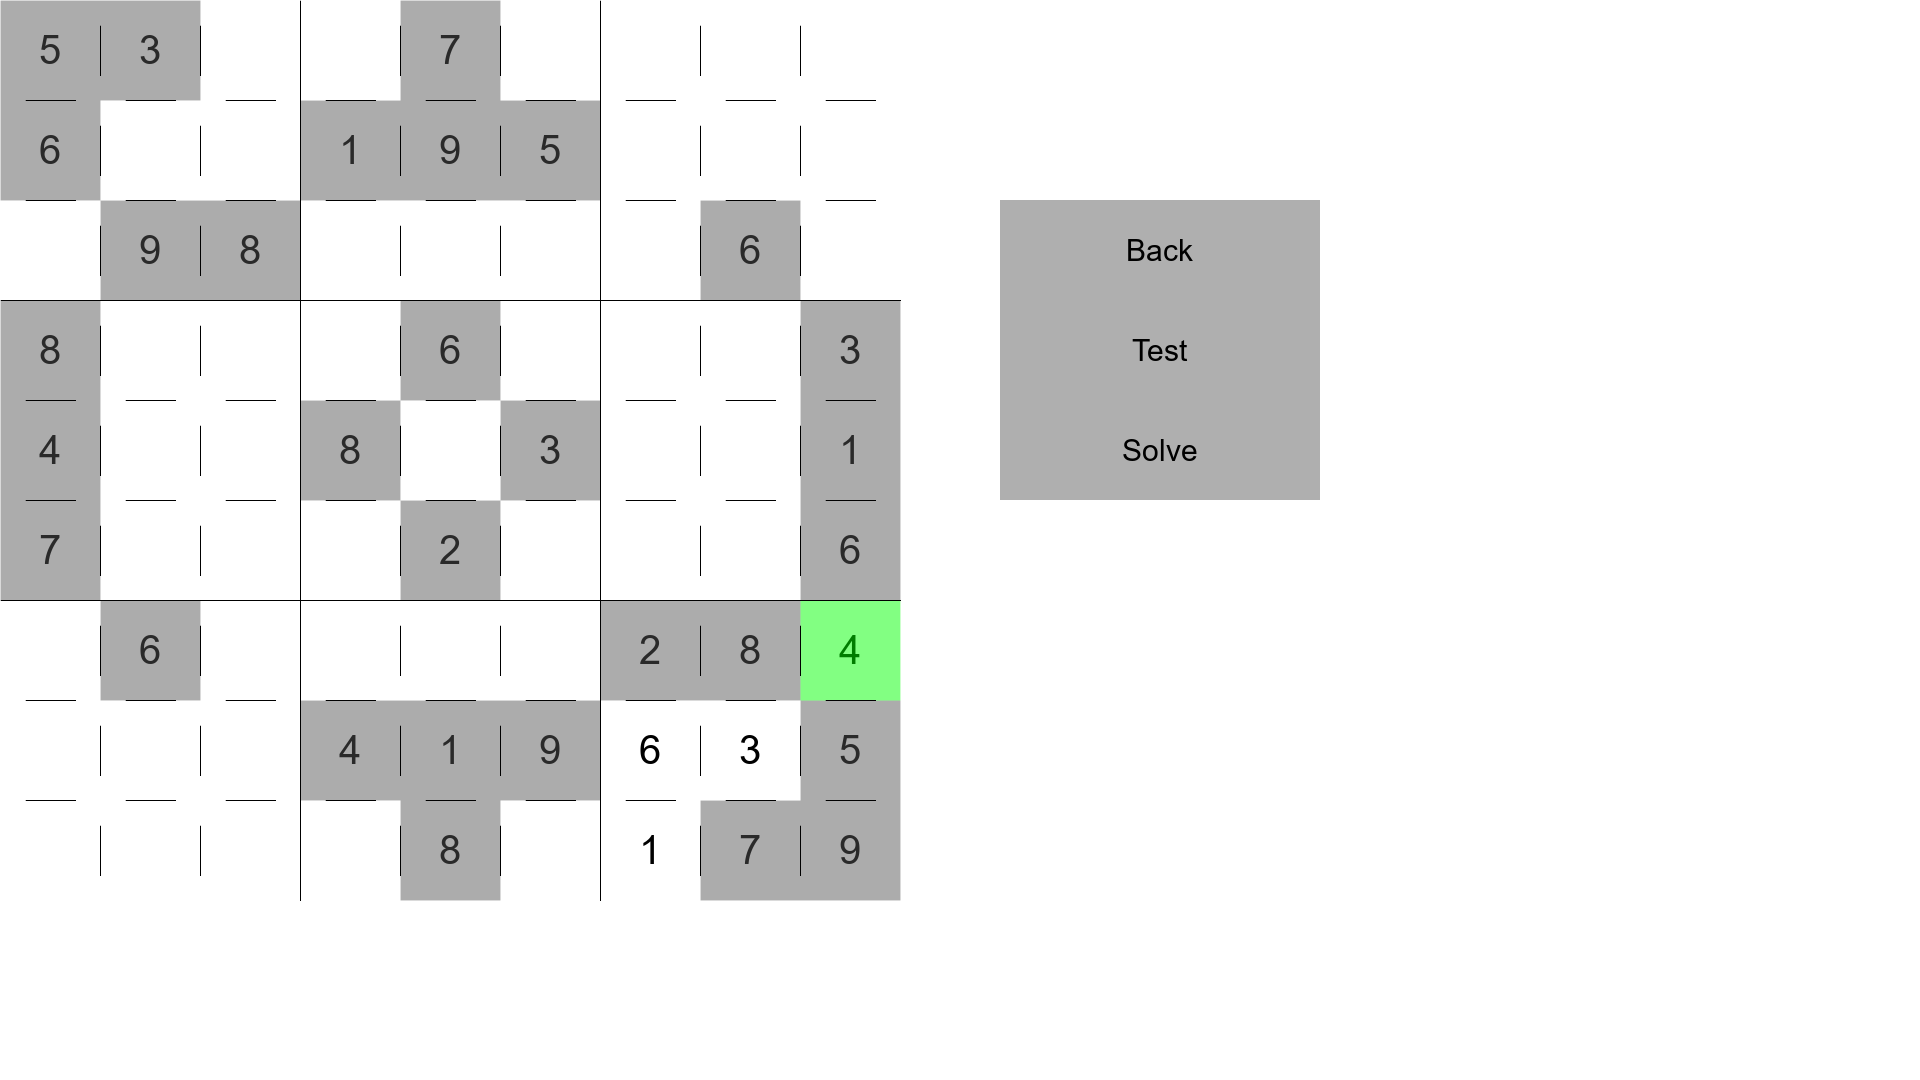
\includegraphics[width=14cm]{user} 
	}
	\caption{\label{fig:user} User Input.}
\end{figure}

\begin{figure}[h]
	\centering
	\fboxsep 2mm
	\framebox{
		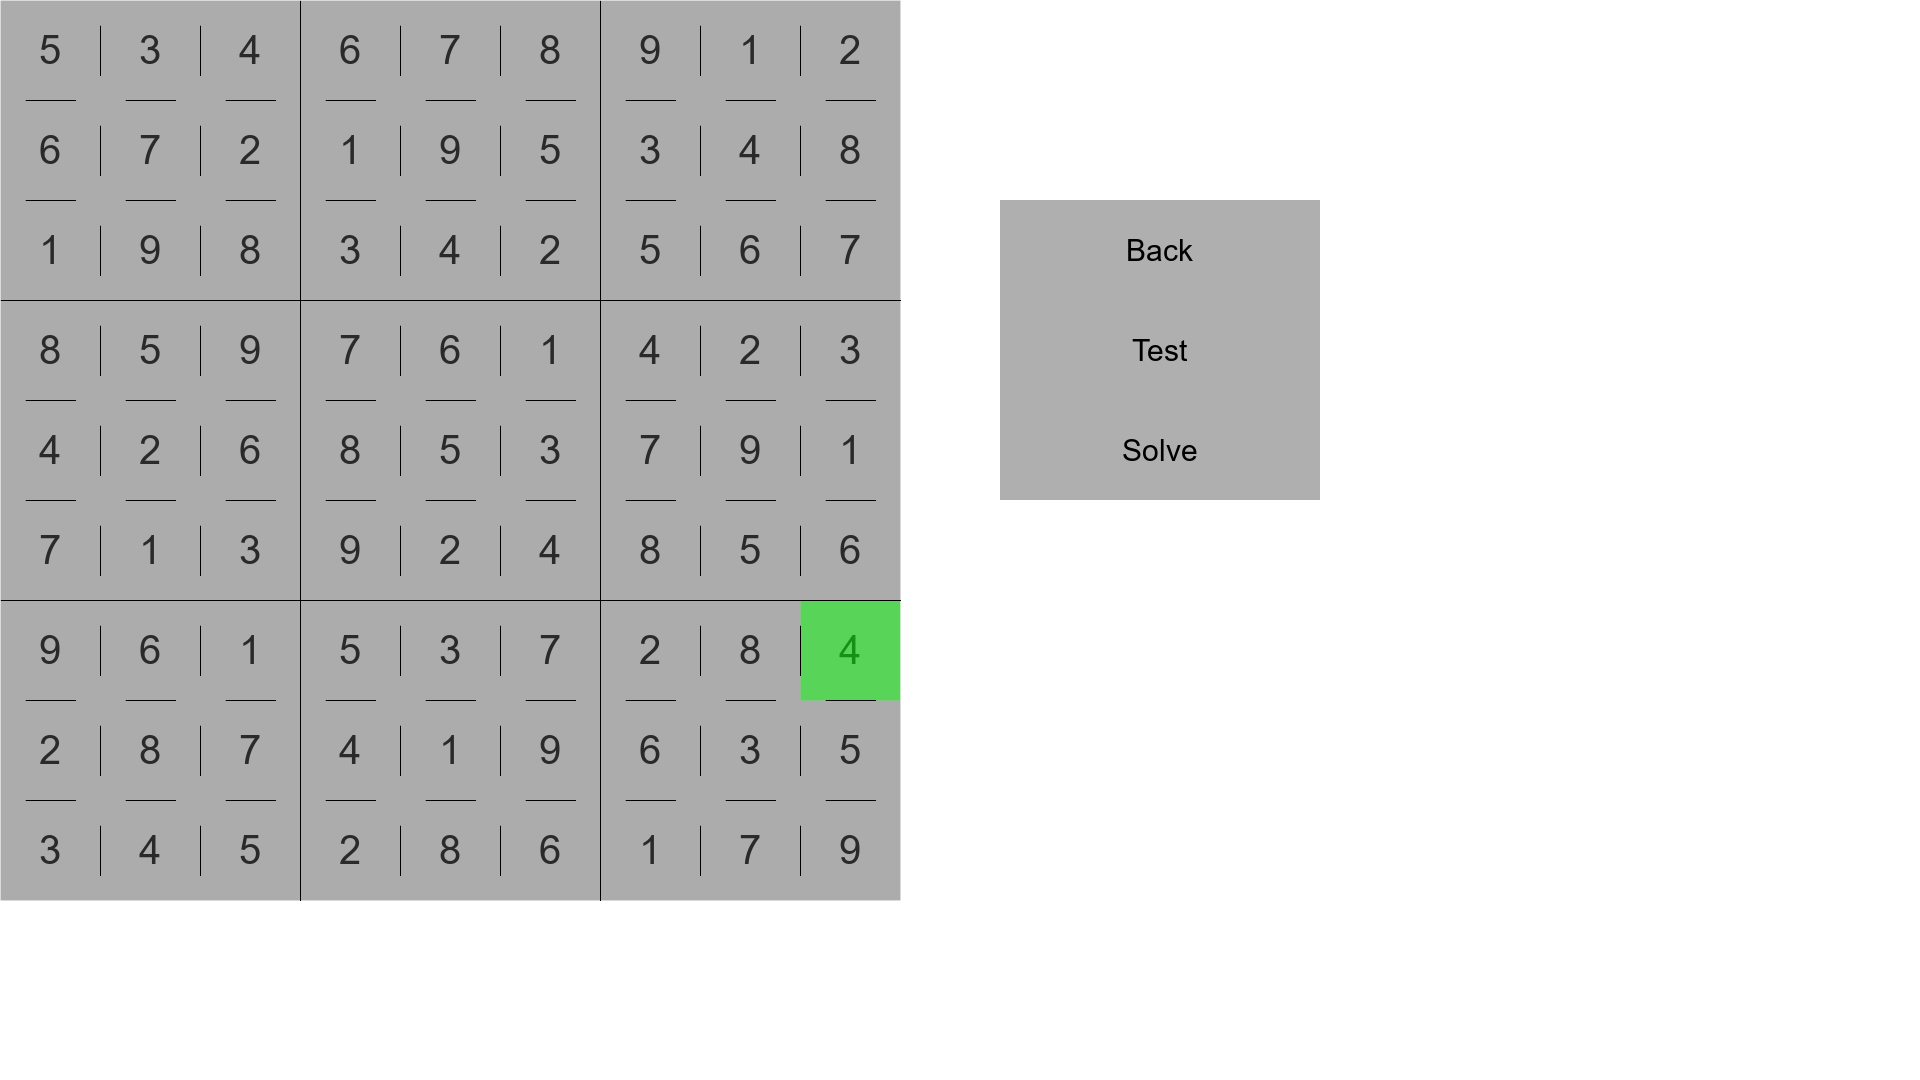
\includegraphics[width=14cm]{solver} 
	}
	\caption{\label{fig:solver} Solver.}
\end{figure}

\label{endpage}



\end{document}

%\end{article}
